\chapter{Arhitektura i dizajn sustava}
		
		
		Arhitekturu možemo podijeliti na tri podsustava (slika \ref{fig:arhitekturaSkica}):

		\begin{packed_item}
			\item  Mobilna aplikacija
			\item  Poslužitelj
			\item  Baza podataka
		\end{packed_item}

		\begin{figure}[H]
			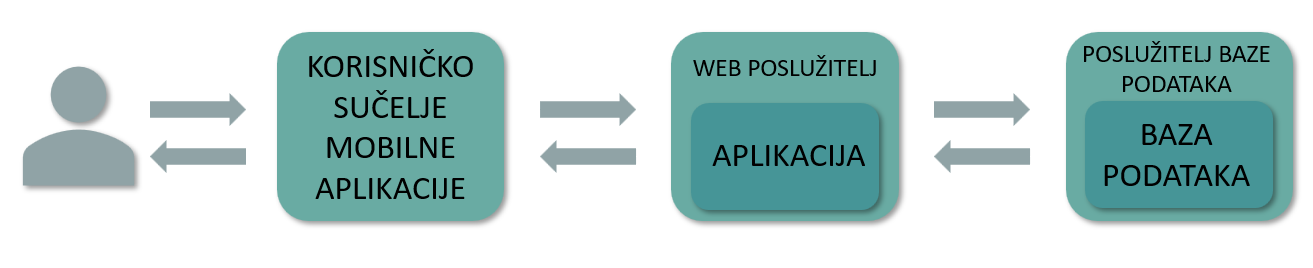
\includegraphics[scale=0.63]{slike/arhitektura.PNG} %veličina slike u odnosu na originalnu datoteku i pozicija slike
			\centering
			\caption{Arhitektura sustava}
			\label{fig:arhitekturaSkica}
		\end{figure}
	
		\textit{\underbar{Korisničko sučelje}} aplikacije korisniku omogućuje pregled i unos podataka u aplikaciju. Sučelje je jednostavno i prilagođeno za jednostavnu uporabu svima. Korisnik preko sučelja šalje zahtjeve na poslužitelj.

		\textit{\underbar{Poslužitelj}} služi za komunikaciju klijenta s aplikacijom. Komunikacija se odvija preko HTTP (engl. \textit{Hyper Text Transfer Protocol}) protokola, što je protokol u prijenosu informacija. Poslužitelj je onaj koji pokreće aplikaciju te joj prosljeđuje zahtjeve.

		\textit{\underbar{Mobilna aplikacija}} obrađuje korisničke zahtjeve, te ovisno o zahtjevu pristupa bazi podataka i preko poslužitelja vraća odgovor korisniku preko .json dokumenta kojeg zatim sučelje prikazuje na način razumljiv svakom korisniku.

		Za izradu naše aplikacije odabrali smo programski jezik Python s FastAPI radnim okvirom te programski jezik Kotlin. Razvojna okruženja koja koristimo su PyCharm za Python i Android Studio za Kotlin.

		Arhitektura aplikacije temeljit će se na MVC (Model-View-Controller) konceptu (slika \ref{fig:mvcSkica}).

		\begin{figure}[H]
			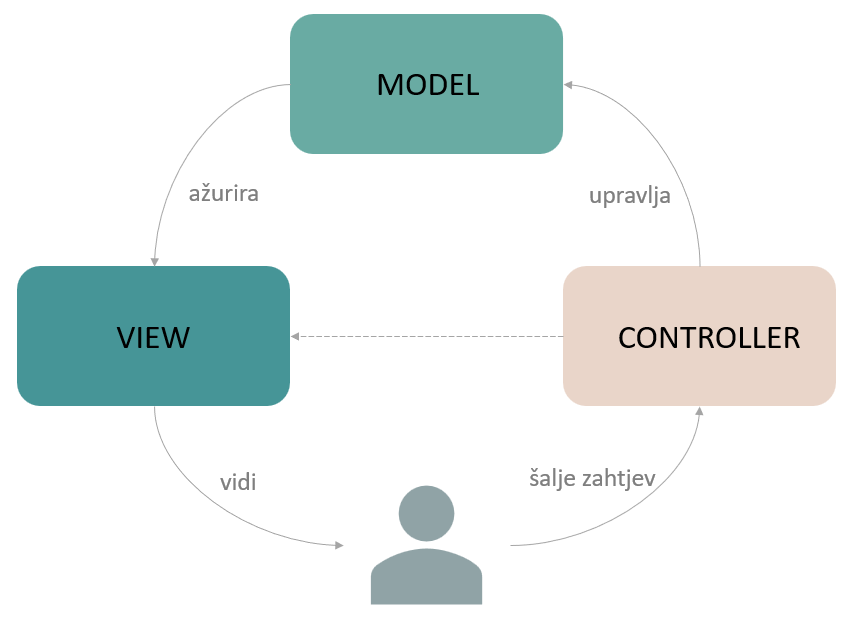
\includegraphics[scale=0.75]{slike/mvc.PNG} %veličina slike u odnosu na originalnu datoteku i pozicija slike
			\centering
			\caption{MVC koncept}
			\label{fig:mvcSkica}
		\end{figure}

		Koncept dijeli aplikaciju na tri sloja – model, view i controller. Svaki sloj izvršava određeni skup zadataka, a svi slojevi djeluju zajedno kako bi ostvarili traženu funkcionalnost aplikacije. Omogućen je nezavisan razvoj pojedinih dijelova čime se pojednostavljuje razvoj i testiranje. 

		\underbar{\textit{Model}} je središnja komponenta ovog koncepta. Upravlja podacima i logikom aplikacije, komunicira s bazom te nema dodira sa sučeljem. Prima zahtjeve od upravljača da se ažurira.

		\underbar{\textit{View}} sadrži komponente aplikacije vidljive korisniku. Omogućuje vizualizaciju podataka spremljenih u modelu i nudi interakciju  korisnikom.

		\underbar{\textit{Controller}}  prima unesene podatke i prevodi ih u naredbe za model i view. Upravlja zahtjevima korisnika i prenosi ih ostalim elementima.
				
		\section{Baza podataka}
			
		 Za potrebe našeg sustava, odabrali smo relacijsku bazu podataka zbog njezine strukture koja olakšava modeliranje stvarnog svijeta. Osnovna građevna jedinica baze je relacija, odnosno tablica koja je identificirana imenom i skupom atributa. Glavna funkcija baze podataka je brza i jednostavna pohrana, izmjena i dohvat podataka za daljnju obradu. Baza podataka naše aplikacije uključuje sljedeće entitete:
		
		\begin{packed_item}
			\item  UserCustom		\textit{~ (korisnik)}
			\item  UserAuth			\textit{~ (prijava za korisnika)}
			\item  Advertisement	\textit{~ (oglas)}
			\item  Pet				\textit{~ (ljubimac)}
			\item  Picture			\textit{~ (slika)}
			\item  Message			\textit{~ (poruka)}
		\end{packed_item}
		
			\subsection{Opis tablica}
			
			
			\textbf{UserCustom}\hspace{10pt}Ovaj entitet sadržava sve važne informacije o korisniku aplikacije.
			Sadrži atribute: id (korisnički identifikacijski broj), username (korisničko ime), isShelter, firstName (ime korisnika), lastName (prezime korisnika), shelterName (ime skloništa ako je riječ o skloništu), email i phoneNumber (broj telefona). Ovaj entitet u vezi je 
			\textit{One-to-One} s entitetom UserAuth preko atributa username (korisničko ime korisnika),
			u vezi \textit{One-to-Many} s Message (poruka) preko korisničkog identifikacijskog broja,
			u vezi \textit{One-to-Many} s entitetom Advertisement preko korisničkog identifikacijskog broja (ili identifikacijskog broja skloništa).
			
				%Svjetlozelenom bojom označite primarni ključ. Svjetlo plavom označite strani ključ
				
				\begin{longtblr}[
					label=none,
					entry=none
					]{
						width = \textwidth,
						colspec={|X[6,l]|X[6, l]|X[20, l]|}, 
						rowhead = 1,
					} %definicija širine tablice, širine stupaca, poravnanje i broja redaka naslova tablice
					\hline \SetCell[c=3]{c}{\textbf{UserCustom}}	 \\ \hline[3pt]
					\SetCell{LightGreen}id & INT	&  jedinstveni brojčani identifikator korisnika	\\ \hline
					username & VARCHAR	&  jedinstveni identifikator korisnika	\\ \hline
					isShelter & BOOLEAN	&  oznaka je li korisnik sklonište	\\ \hline
					firstName & VARCHAR	&  ime korisnika	\\ \hline
					lastName & VARCHAR	&  prezime korisnika	\\ \hline
					shelterName & VARCHAR	&  ime skloništa	\\ \hline
					email & EMAIL \textit{(definirano u bazi podataka)}	&  e-mail adresa korisnika	\\ \hline
					phoneNumber & VARCHAR	&  broj telefona korisnika	\\ \hline
				\end{longtblr}
				
			\textbf{UserAuth}\hspace{10pt}Ovaj entitet sadržava sve što je potrebno kako bi se u sustav prijavio korisnik, a to je njegov username (korisničko ime) i password (pripadajuća loznika).Ovaj entitet je u vezi
			\textit{One-to-One} s entitetom UserCustom preko atributa username (korisničko ime).
			
				\begin{longtblr}[
					label=none,
					entry=none
					]{
						width = \textwidth,
						colspec={|X[6,l]|X[6, l]|X[20, l]|}, 
						rowhead = 1,
					} %definicija širine tablice, širine stupaca, poravnanje i broja redaka naslova tablice
					\hline \SetCell[c=3]{c}{\textbf{UserAuth}}	 \\ \hline[3pt]
					\SetCell{LightBlue}	username & VARCHAR &  jedinstveni identifikator korisnika  	\\ \hline
					password & VARCHAR	&  hash lozinke	\\ \hline
				\end{longtblr}
				
			
			\textbf{Advertisement}\hspace{10pt}Ovaj entitet sadržava sve važne informacije o oglasima koje će korisnici moći postavljati ili čitati.
			Sadrži atribute: id (identifikacijski broj oglasa), category (kategoriju), deleted (podatak o tome je li oglas izbrisan), dateTimeAdv (vrijeme oglašavanja), isInShelter (podatak o tome je li oglas ljubimca označen da je u skloništu), userId (ID korisnika), petId (ID ljubimca) i shelterId (ID skloništa).
			Ovaj entitet je u vezi
			\textit{Many-to-One} s entitetom UserCustom preko atributa userId i shelterId,
			u vezi \textit{One-to-Many} s entitetom Message preko identifikacijskog broja oglasa,
			u vezi \textit{One-to-Many} s entitetom Picture također preko identifikacijskog broja oglasa
			te u vezi \textit{One-to-One} s entitetom Pet (ljubimcem) preko identifikacijskog broja ljubimca.
			
				\begin{longtblr}[
					label=none,
					entry=none
					]{
						width = \textwidth,
						colspec={|X[6,l]|X[6, l]|X[20, l]|}, 
						rowhead = 1,
					} %definicija širine tablice, širine stupaca, poravnanje i broja redaka naslova tablice
					\hline \SetCell[c=3]{c}{\textbf{Advertisement}}	 \\ \hline[3pt]
					\SetCell{LightGreen}	id & INT &  jedinstveni brojčani identifikator oglasa	\\ \hline
					category & ENUM	&  kategorije: lost, found, abandoned, sheltered, dead	\\ \hline
					deleted & BOOLEAN	&  oznaka je li oglas izbrisan	\\ \hline
					dateTimeAdv & TIMESTAMP	&  vrijeme postavljanja oglasa	\\ \hline
					isInShelter & BOOLEAN	&  oznaka je li ljubimac smješten u sklonište	\\ \hline
					\SetCell{LightBlue} userId & INT	&  jedinstveni brojčani identifikator korisnika	\\ \hline
					\SetCell{LightBlue} petId & INT	&  jedinstveni brojčani identifikator ljubimca	\\ \hline
					\SetCell{LightBlue} shelterId & INT	&  jedinstveni brojčani identifikator skloništa	\\ \hline
				\end{longtblr}
				
				
			\textbf{Pet}\hspace{10pt}Ovaj entitet sadržava sve važne informacije o nestalom ljubimcu koje će biti od pomoći pri potrazi.
			Sadrži atribute: id (identifikacijski broj ljubimca), species (vrsta ljubimca), name (ime), color (boja), dateTimeLost (vrijeme kad je ljubimac izgubljen), locationLost (lokacija na kojoj je izgubljen) i description (opis).
			Ovaj entitet je u vezi
			\textit{One-to-One} s entitetom Advertisement  preko atributa identifikacijskog broja ljubimca.
			
				\begin{longtblr}[
					label=none,
					entry=none
					]{
						width = \textwidth,
						colspec={|X[6,l]|X[6, l]|X[20, l]|}, 
						rowhead = 1,
					} %definicija širine tablice, širine stupaca, poravnanje i broja redaka naslova tablice
					\hline \SetCell[c=3]{c}{\textbf{Pet}}	 \\ \hline[3pt]
					\SetCell{LightGreen} id & INT &  jedinstveni brojčani identifikator ljubimca	\\ \hline
					species & ENUM	& vrsta životinje	\\ \hline
					name & VARCHAR	&  ime ljubimca	\\ \hline
					color & VARCHAR	&  boja ljubimca	\\ \hline
					age & INT	&  starost ljubimca	\\ \hline
					dateTimeLost & TIMESTAMP	&  vrijeme kad je ljubimac izgubljen	\\ \hline
					locationLost & VARCHAR	&  opisuje lokaciju na kojoj je ljubimac izgubljen	\\ \hline
					description & TEXT	&  sve dodatne informacije o ljubimcu	\\ \hline
				\end{longtblr}
				
			
			\textbf{Picture}\hspace{10pt}Ovaj entitet omogućava pohranu i korištenje slika koje se koriste pri potrazi za ljubimcima.
			Sadrži atribute: id (identifikacijski broj slike), link, advertId (identifikacijski broj oglasa) i messageId (identifikacijski broj poruke)
			Ovaj entitet je u vezi
			\textit{Many-to-One} s entitetom Advertisement preko atributa identifikacijskog broja ljubimca te je u vezi
			\textit{Many-to-One} s entitetom Message preko ID-a poruke.
			
				\begin{longtblr}[
					label=none,
					entry=none
					]{
						width = \textwidth,
						colspec={|X[6,l]|X[6, l]|X[20, l]|}, 
						rowhead = 1,
					} %definicija širine tablice, širine stupaca, poravnanje i broja redaka naslova tablice
					\hline \SetCell[c=3]{c}{\textbf{Picture}}	 \\ \hline[3pt]
					\SetCell{LightGreen} id & INT &  jedinstveni brojčani identifikator slike	\\ \hline
					link & VARCHAR	& poveznica prema slici	\\ \hline
					\SetCell{LightBlue} advertId & INT	&  jedinstveni brojčani identifikator oglasa \\ \hline
					\SetCell{LightBlue} messageId & INT	&  jedinstveni brojčani identifikator poruke \\ \hline
				\end{longtblr}
				
				
			\textbf{Message}\hspace{10pt}Ovaj entitet sadržava sve važne informacije tijekom komunikacije korisnika prilikom potrage za nestalim ljubimcima.
			Sadrži atribute: id (identifikacijski broj poruke), text, location (lokaciju), dateTimeMess (vrijeme slanja poruke), advertId (ID oglasa) i userId (ID korisnika koji je poslao poruku).
			Ovaj entitet je u vezi
			\textit{Many-to-One} s entitetom UserCustom preko atributa identifikacijskog broja korisnika, u vezi
			\textit{Many-to-One} s entitetom Advertisement preko ID-a oglasa te je u vezi
			\textit{Many-to-One} s entitetom Picture preko identifikacijskog broja poruke.
			
				\begin{longtblr}[
					label=none,
					entry=none
					]{
						width = \textwidth,
						colspec={|X[6,l]|X[6, l]|X[20, l]|}, 
						rowhead = 1,
					} %definicija širine tablice, širine stupaca, poravnanje i broja redaka naslova tablice
					\hline \SetCell[c=3]{c}{\textbf{Message}}	 \\ \hline[3pt]
					\SetCell{LightGreen} id & INT &  jedinstveni brojčani identifikator poruke	\\ \hline
					text & TEXT	& tekstualni dio poruke	\\ \hline
					location & VARCHAR	& lokacija koju korisnik može poslati	\\ \hline
					dateTimeMess & TIMESTAMP	& vrijeme slanja poruke	\\ \hline
					\SetCell{LightBlue} advertId & INT	&  jedinstveni brojčani identifikator oglasa \\ \hline
					\SetCell{LightBlue} userId & INT	&  jedinstveni brojčani identifikator korisnika \\ \hline
				\end{longtblr}
			
			
				
			
			\subsection{Dijagram baze podataka}
				
				%unos slike
				\begin{figure}[H]
					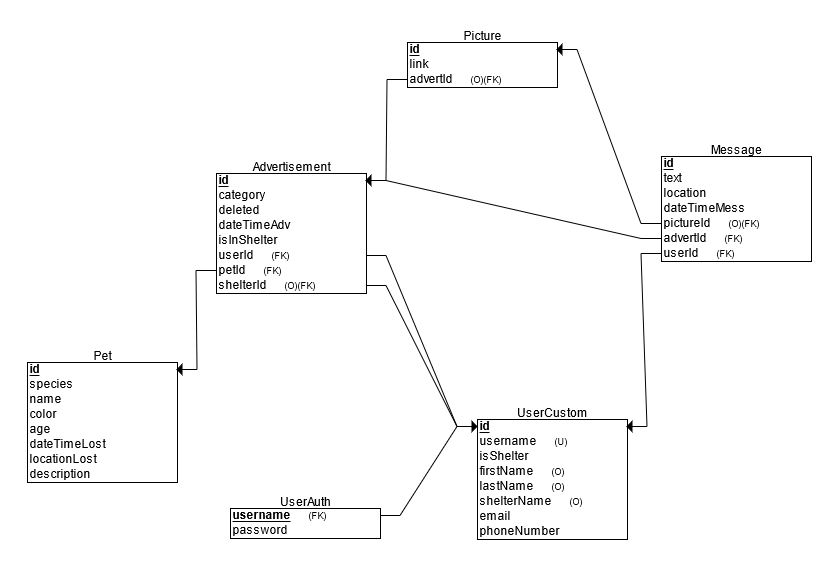
\includegraphics[scale=0.63]{dijagrami/dijagramBaze/relacijskiModel.PNG} %veličina slike u odnosu na originalnu datoteku i pozicija slike
					\centering
					\caption{Relacijski dijagram baze podataka}
					\label{fig:relDijagram}
				\end{figure}

				\begin{figure}[H]
					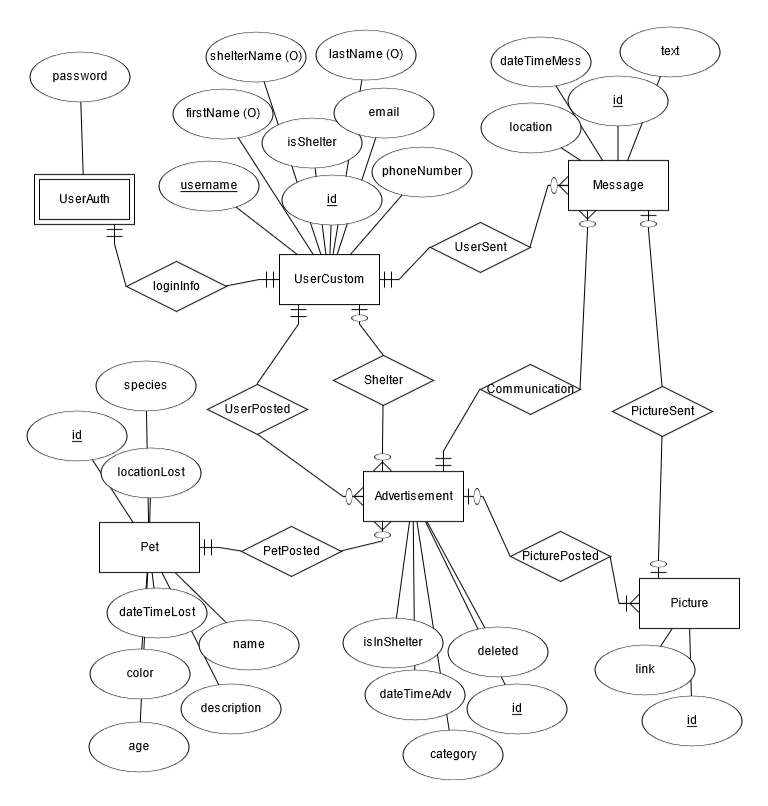
\includegraphics[scale=0.65]{dijagrami/dijagramBaze/ERmodel.PNG} %veličina slike u odnosu na originalnu datoteku i pozicija slike
					\centering
					\caption{E-R dijagram baze podataka}
					\label{fig:erDijagram}
				\end{figure}

			\eject
			
			
		\section{Dijagram razreda}
		
			Na slikama \ref{fig:drModels}, \ref{fig:drDataTransferObjects}, \ref{fig:drRepository} i \ref{fig:drControllers} su prikazani razredi koji pripadaju \textit{backend} dijelu MVC arhitekture. Na slici \ref{fig:drView} prikazani su razredi \textit{frontend} dijela arhitekture. Razredi prikazani na slici \ref{fig:drRepository} prikazuju \textit{Repository} koji je zadužen za interakciju s bazom. Razredi na slici \ref{fig:drControllers} nasljeđuju razred \textit{APIRouter}. Metode implementirane u tim razredima manipuliraju s DTO \textit{(Data transfer object)}, a oni su dohvaćeni pomoću metoda implementiranih u Model razredima.

			Zbog lakše organizacije, razredi su podijeljeni logički po pravu pristupa metodama određenih aktora. Prikazane su isključivo ovisnosti između razreda koji pripadaju istom dijelu dijagrama. Ostale ovisnosti mogu se zaključiti iz naziva i tipova atributa u razredima.

			\begin{figure}[H]
				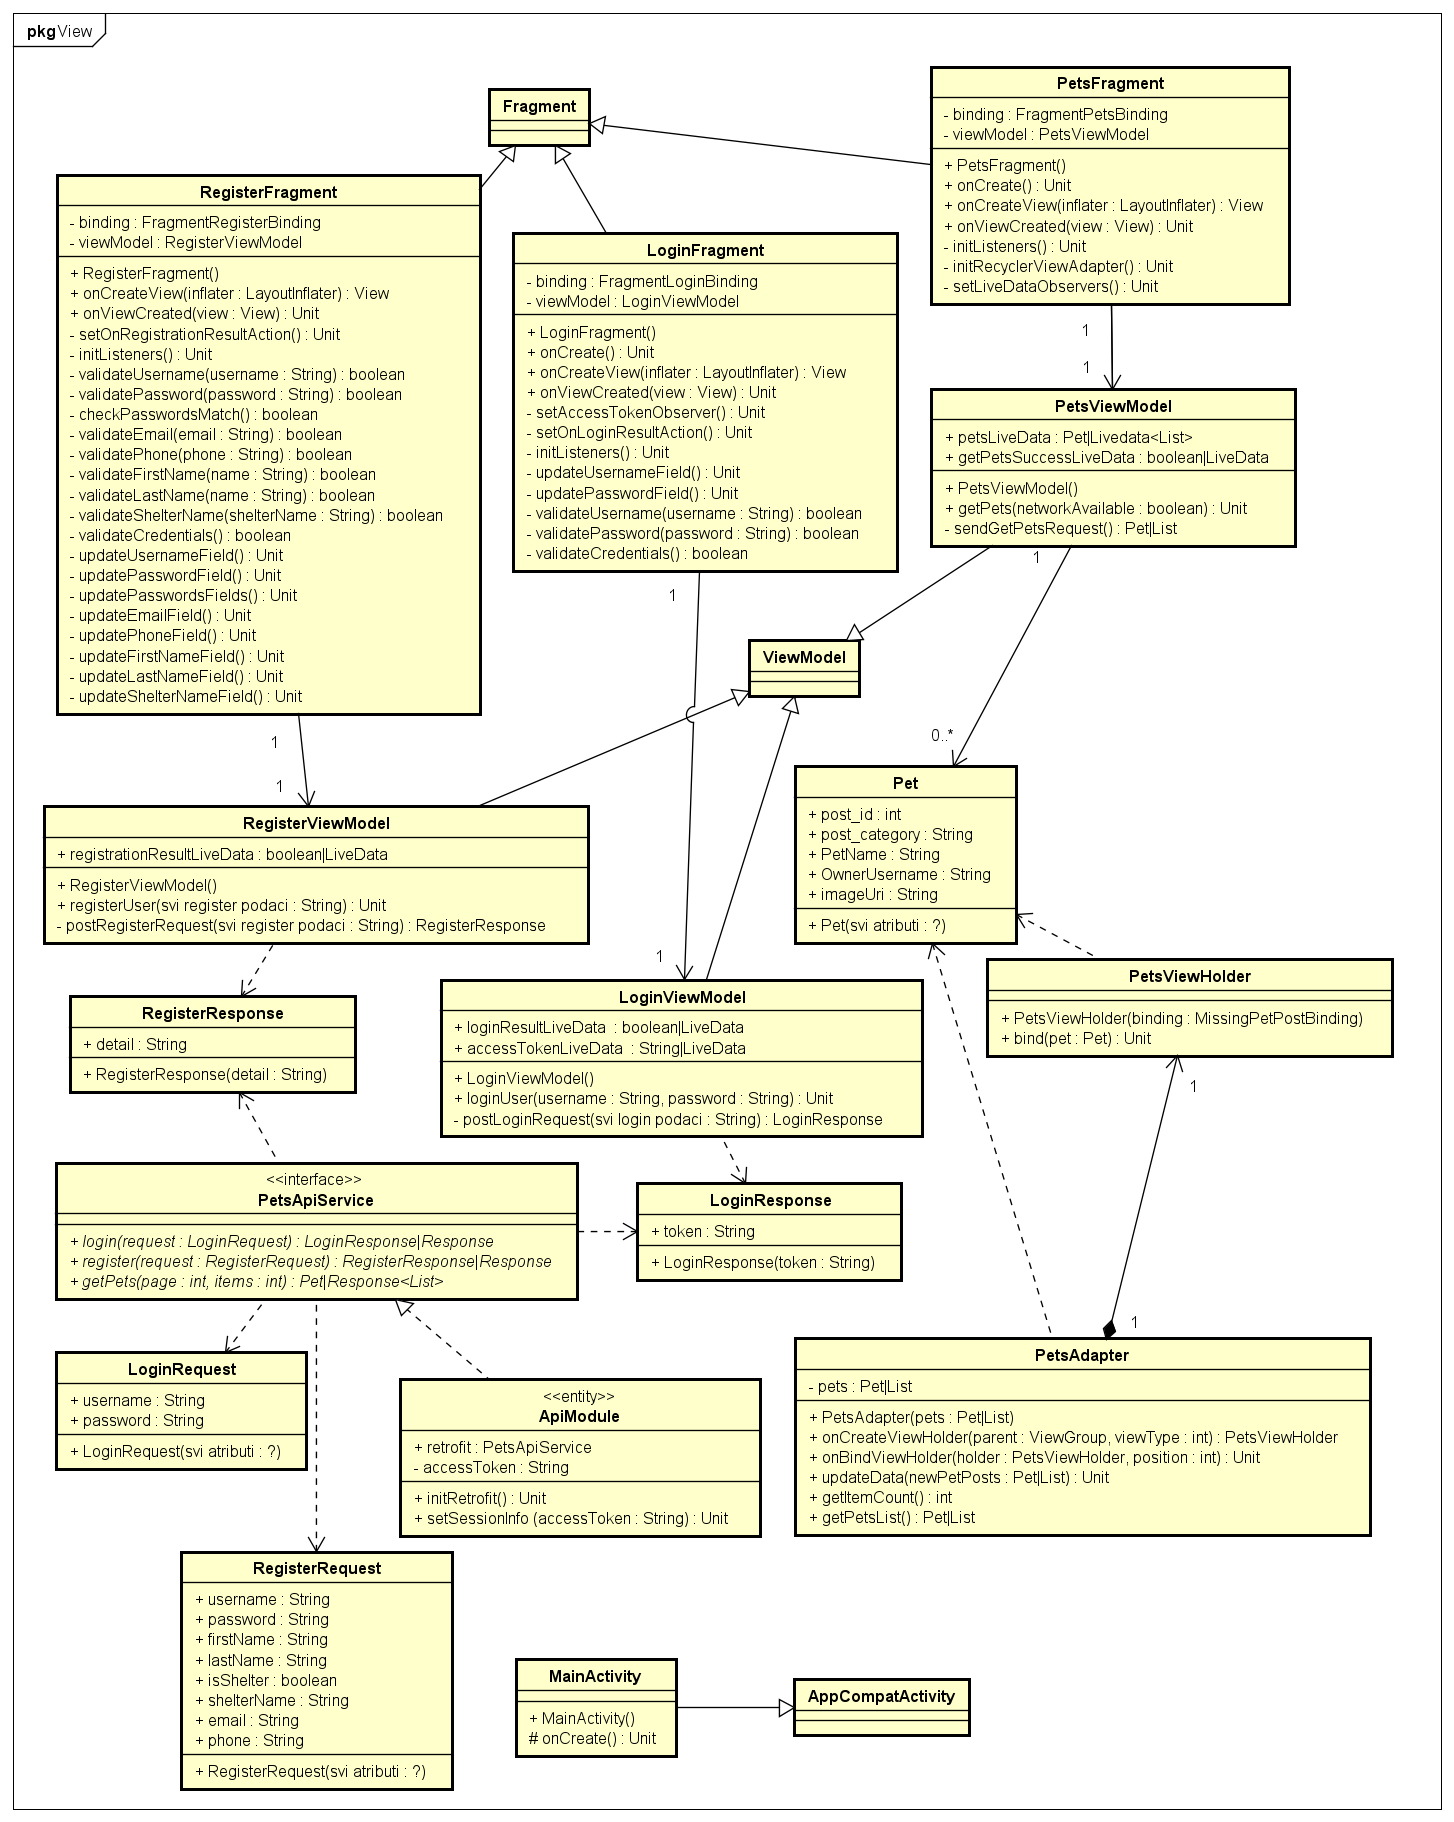
\includegraphics[scale=0.45]{dijagrami/dijagramiRazreda/View.PNG} %veličina slike u odnosu na originalnu datoteku i pozicija slike
				\centering
				\caption{Dijagram razreda - dio View}
				\label{fig:drView}
			\end{figure}

			Model razredi preslikavaju strukturu baze podataka u aplikaciji. Implementirane metode direktno komuniciraju s bazom podataka te vraćaju tražene podatke. Razred UserCustom predstavlja registriranog korisnika koji ima pristup svim stavkama aplikacije. Razred UserAuth predstavlja podatke za prijavu registriranog korisnika. Razred Advertisement predstavlja objavljeni oglas. Pet je razred koji sadrži unesene podatke o nestalom ljubimcu. Razred message predstavlja poruke vezane za komunikaciju o potrazi. Razred Picture predstavlja sliku koja se nalazi ili u oglasu ili u poruci. PetSpecies je enumeracija s mogućim vrstama ljubimca, a AdvertisementCategory enumeracija s kategorijama oglasa.

			\begin{figure}[H]
				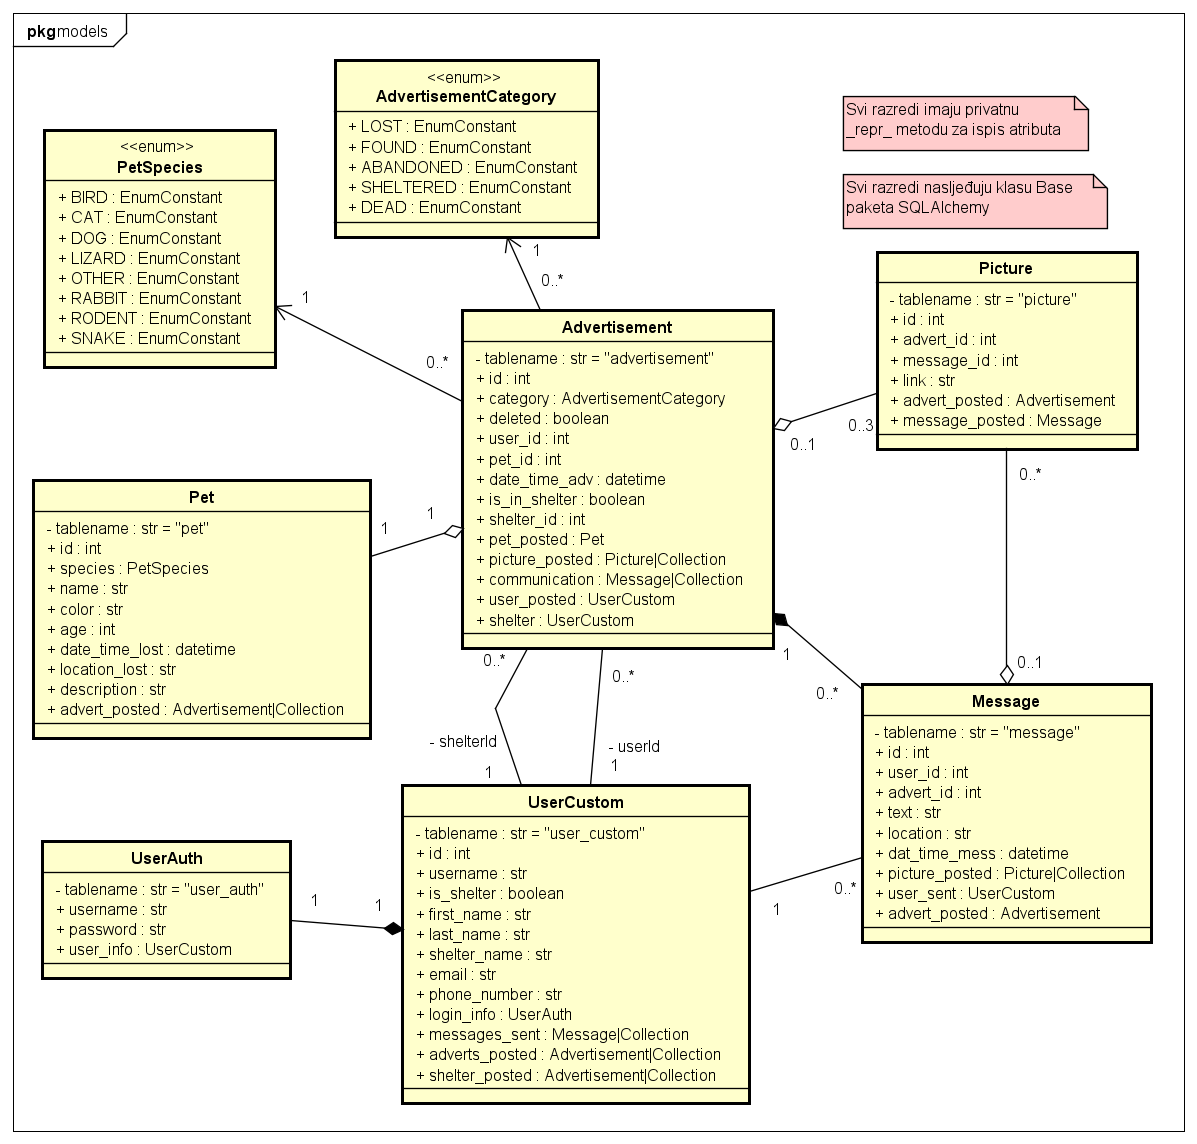
\includegraphics[scale=0.55]{dijagrami/dijagramiRazreda/Models.PNG} %veličina slike u odnosu na originalnu datoteku i pozicija slike
				\centering
				\caption{Dijagram razreda - dio Models}
				\label{fig:drModels}
			\end{figure}
			
			\begin{figure}[H]
				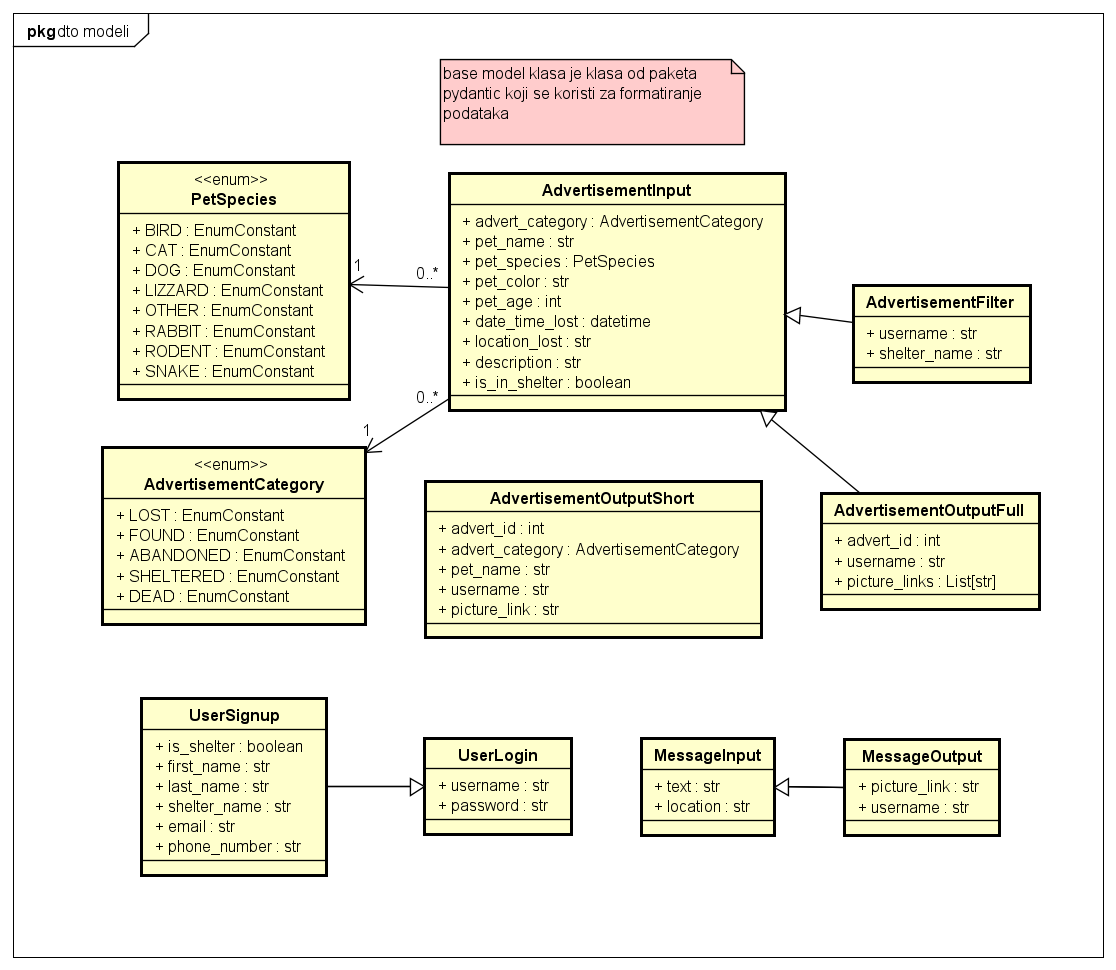
\includegraphics[scale=0.55]{dijagrami/dijagramiRazreda/dto.PNG} %veličina slike u odnosu na originalnu datoteku i pozicija slike
				\centering
				\caption{Dijagram razreda - dio Data transfer objects}
				\label{fig:drDataTransferObjects}
			\end{figure}
			
			\begin{figure}[H]
				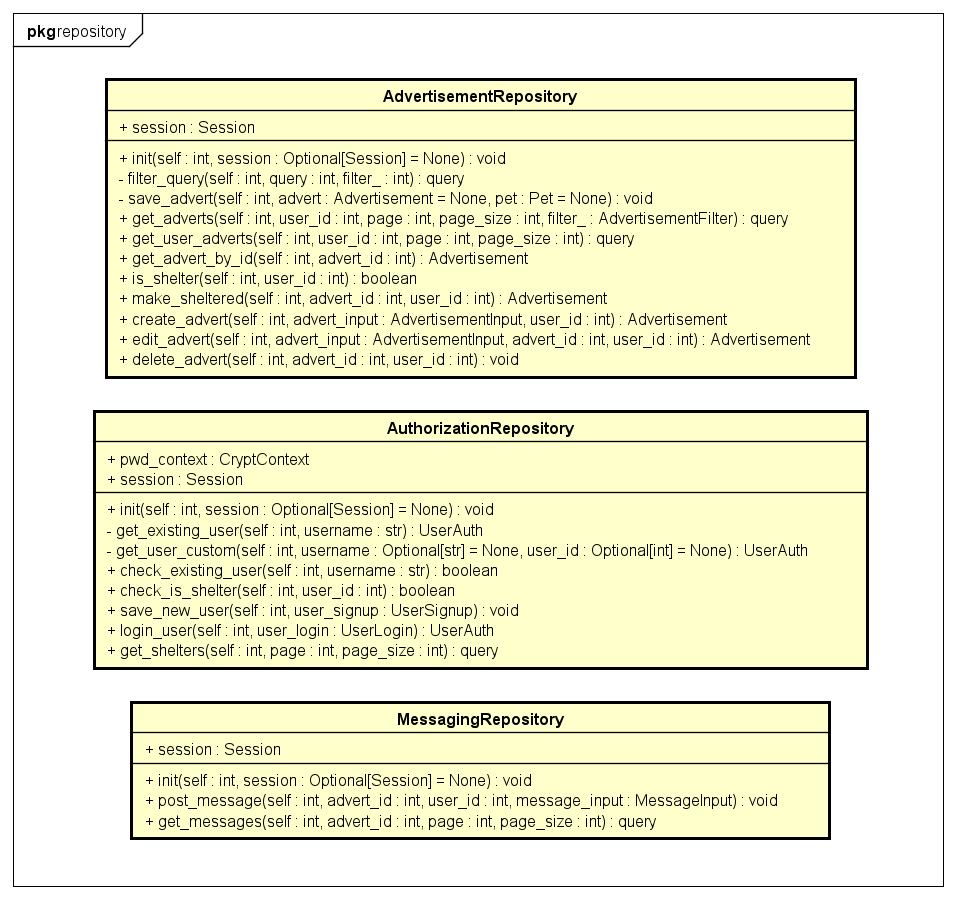
\includegraphics[scale=0.6]{dijagrami/dijagramiRazreda/repo.PNG} %veličina slike u odnosu na originalnu datoteku i pozicija slike
				\centering
				\caption{Dijagram razreda - dio Repository}
				\label{fig:drRepository}
			\end{figure}

			\begin{figure}[H]
				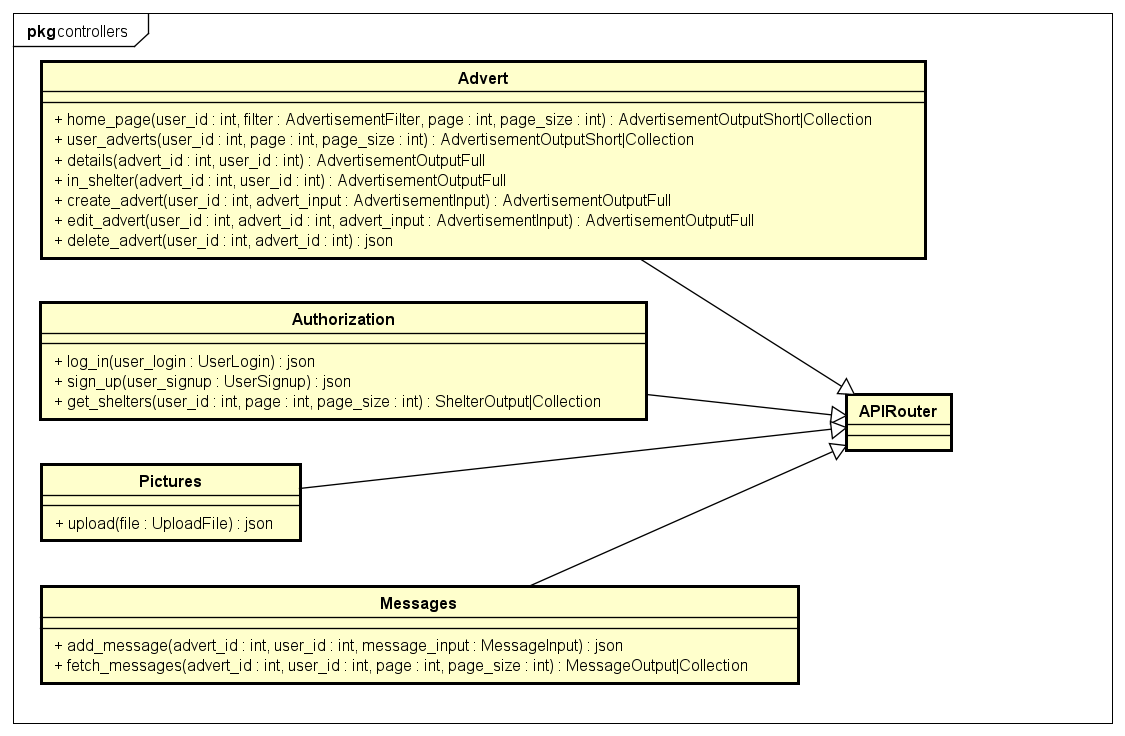
\includegraphics[scale=0.6]{dijagrami/dijagramiRazreda/Controllers.PNG} %veličina slike u odnosu na originalnu datoteku i pozicija slike
				\centering
				\caption{Dijagram razreda - dio Controllers}
				\label{fig:drControllers}
			\end{figure}
			
			\eject
		
		\section{Dijagram stanja}
			
			
			Koristeći aplikaciju korisnik prelazi iz jednog stanja u drugo. Prijelaz iz stanja prikazuje se na dijagramu. Na slici \ref{fig:dStanja} nalazi se dijagram stanja za klijenta aplikacije. Nakon što korisnik obavi prijavu, prikazuje mu se početna stranica na kojoj može listati oglase. S pomoću jasno definiranih tipki lako se može navigirati kroz aplikaciju odabirući nekoliko mogućnosti. Može objaviti novi oglas, pregledati svoj profil, vidjeti sve vlastite oglase ili pretražiti postojeće oglase.
			
			\begin{figure}[H]
				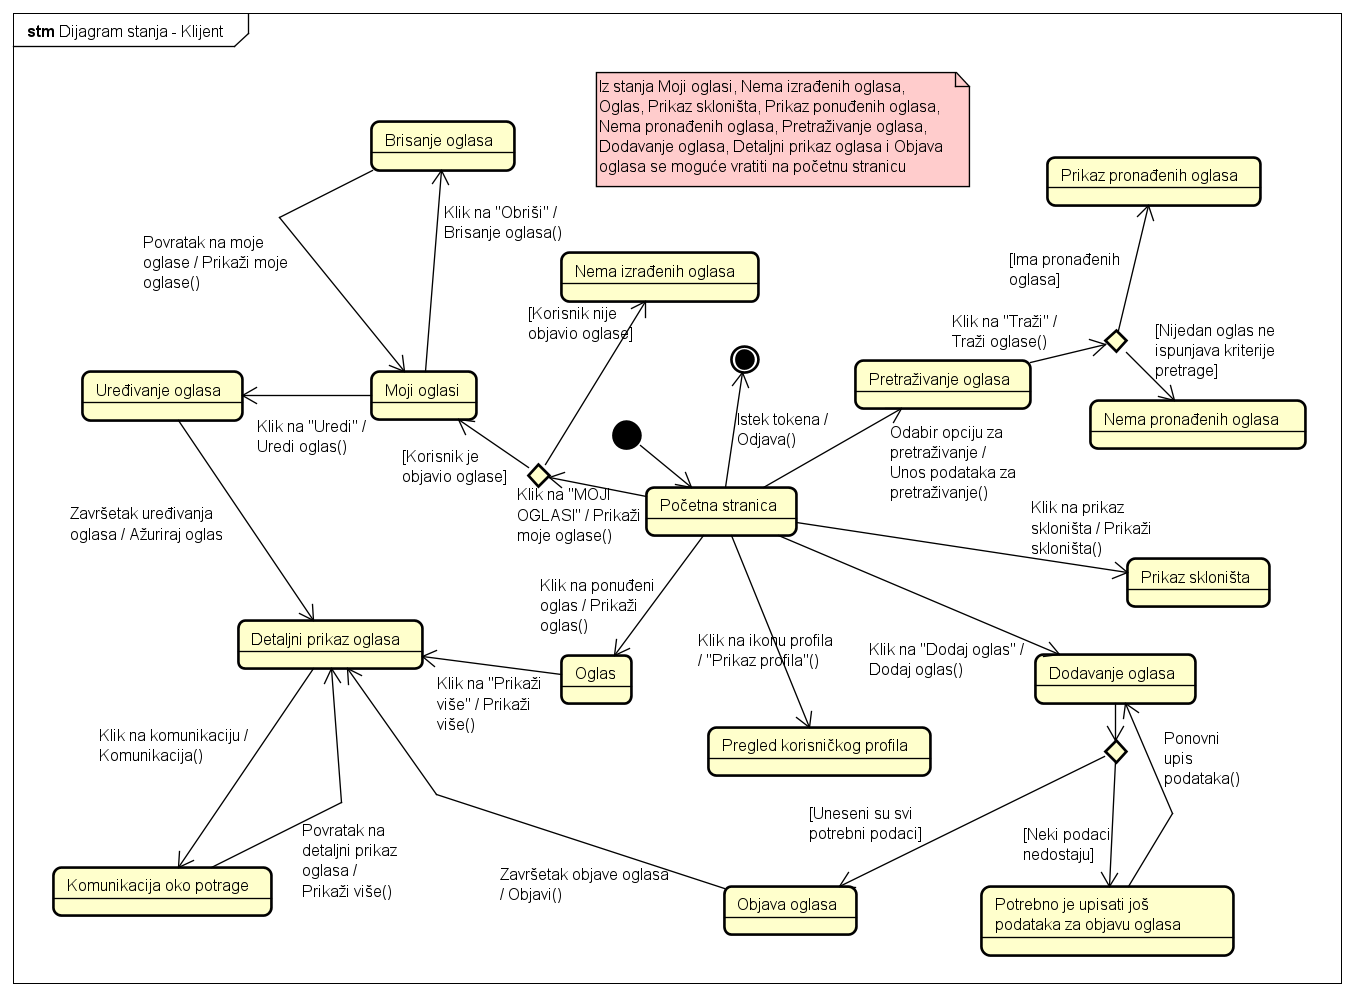
\includegraphics[scale=0.5]{dijagrami/dijagramStanja/dijagramStanja.PNG} %veličina slike u odnosu na originalnu datoteku i pozicija slike
				\centering
				\caption{Dijagram stanja}
				\label{fig:dStanja}
			\end{figure}
			
			\eject 
		
		\section{Dijagram aktivnosti}

			UML-dijagrami aktivnosti su ponašajni UML-dijagrami koji se upotrebljavaju za modeliranje i vizualizaciju dinamičkog ponašanja sustava. Prikazuju tijek aktivnosti, akcija i odluka procesa u sustavu. Svaki novi korak ovisi o završetku i rezultatu prethodnog. Na dijagramu \ref{fig:dAktivnosti} prikazan je proces kreiranja novog oglasa za nestalog ljubimca. Korisnik se prvo prijavljuje u sustav, a zatim odabire opciju za objavu novog oglasa. Unosi željene podatke o ljubimcu koji se onda provjeravaju u aplikaciji i na bazi. Ako su neispravni aplikacija traži ponovni unos, inače se spremaju u bazu. Novi oglas se zatim prikazuje korisniku.
			
			\begin{figure}[H]
				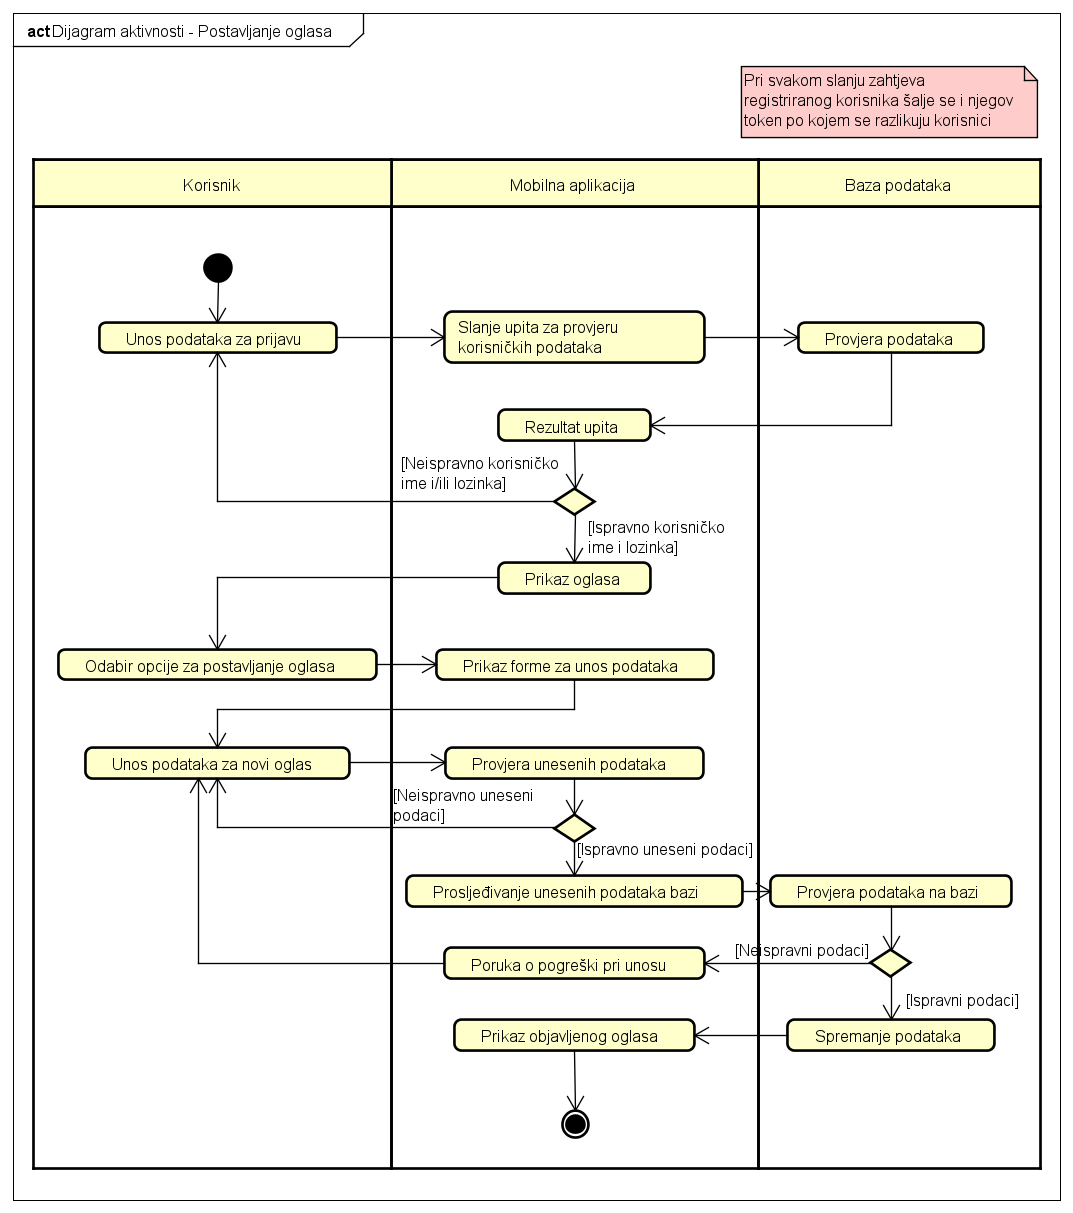
\includegraphics[scale=0.6]{dijagrami/dijagramAktivnosti/dAktivnosti.PNG} %veličina slike u odnosu na originalnu datoteku i pozicija slike
				\centering
				\caption{Dijagram aktivnosti - Postavljanje oglasa}
				\label{fig:dAktivnosti}
			\end{figure}
			
			\eject
		\section{Dijagram komponenti}
		
			\begin{figure}[H]
				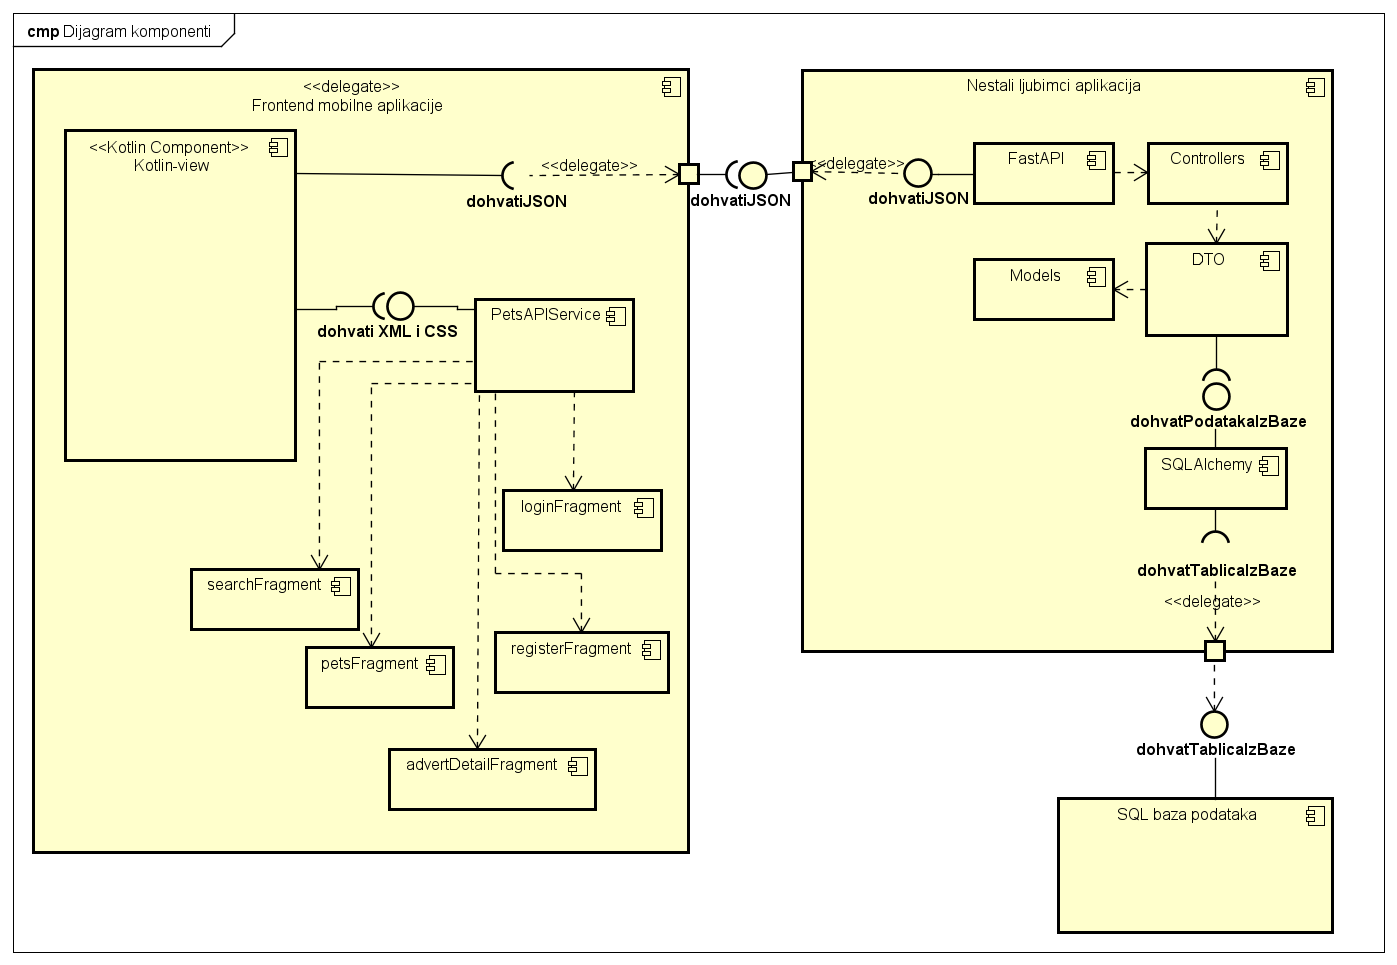
\includegraphics[scale=0.48]{dijagrami/dijagramKomponenti/dKomponenti.PNG} %veličina slike u odnosu na originalnu datoteku i pozicija slike
				\centering
				\caption{Dijagram komponenti}
				\label{fig:dKomponenti}
			\end{figure}
